\begin{figure}[ht]
    \centering
    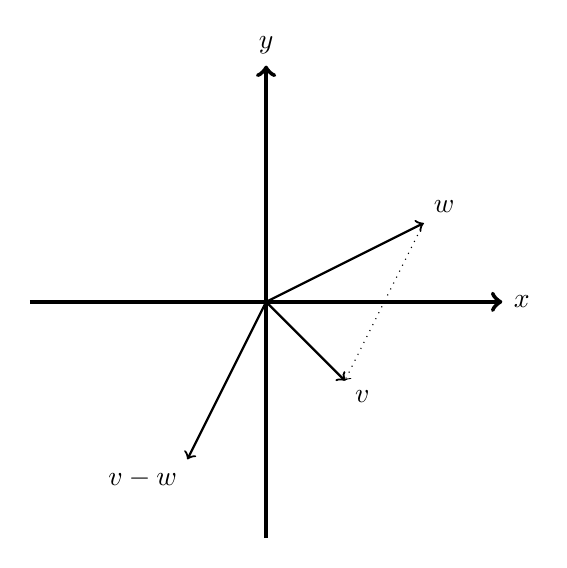
\begin{tikzpicture}
    \draw[->,ultra thick] (-3,0)--(3,0) node[right]{$x$};
    \draw[->,ultra thick] (0,-3)--(0,3) node[above]{$y$};
    % Vetor v
    \draw[->,thick] (0,0) -- (2,1) node[above right]{$w$};
    % Vetor v-w
    \draw[->,thick] (0,0) -- (-1,-2) node[below left]{$v-w$};
    \draw[->,dotted] (2,1) -- (1,-1);
    % Vetor v+w
    \draw[->,thick] (0,0) -- (1,-1) node[below right]{$v$};
    \end{tikzpicture}
    \caption{O vetor $v-w$ como deslocamento da extremidade de $w$ até a extremidade de $v$.}
    \label{fig:diferenca-vetores}
\end{figure}
